% More info on this class can be found on: http://www.ctan.org/pkg/paper.
\documentclass[12pt,a4paper,oneside]{paper} % Accepts option `twocolumn`.
%\usepackage{fullpage} % If needed.
\usepackage{lmodern} % Fonts. Needed somehow, otherwise things break.
\usepackage[english]{babel} % English language/hyphenation.
\usepackage[T1]{fontenc} % Use 8-bit output encoding.
\usepackage[utf8]{inputenc} % Can use UTF-8 in the source files.
\usepackage[babel]{microtype} % Improves appearance of text.
\usepackage{url}
\usepackage{csquotes}
\usepackage{amsmath,amsthm, amssymb}
% Reference sheet: http://merkel.zoneo.net/Latex/natbib.php
\usepackage{natbib} % Better references
\bibliographystyle{abbrvnat}
% If possible, it is preferable to directly include PDF images.
\usepackage{graphicx}
\graphicspath{{fig/}} 
\usepackage{hyperref}
\hypersetup{colorlinks=true}


\title{On the First Eigenvalue of the Graph}
\subtitle{Optional subtitle}
\author{Lucas Maystre \and Super Visor\thanks{School of Computer and
Communication Sciences, EPFL, Switzerland. Corresponding author: Lucas Maystre,
\href{mailto:email@epfl.ch}{\nolinkurl{email@epfl.ch}}.}}

% Don't know how this is used. Removing it messes the header.
\shortauthor{Maystre}
\shorttitle{Eigenvalues}

\begin{document}
\maketitle

\abstract{
Lorem ipsum dolor sit amet, consectetur adipiscing elit. In aliquam rutrum erat
sed bibendum. Vestibulum consectetur nisi id arcu hendrerit viverra. Etiam
venenatis sapien id lacus adipiscing, at vehicula mi euismod. Suspendisse non
condimentum erat, quis molestie quam.
}


%%%%%%%%%%%%%%%%%%%%%%%%%%%%%%%%%%%%%%%%%%%%%%%%%%%%%%%%%%%%%%%%%%%%%%%%%
\section{Introduction} %%%%%%%%%%%%%%%%%%%%%%%%%%%%%%%%%%%%%%%%%%%%%%%%%%
\label{sec:intro}

Nunc non nunc eget elit ullamcorper scelerisque non quis sem. Vivamus eu
venenatis diam. Integer vitae diam at risus pharetra malesuada. Vestibulum
congue lorem cursus tellus accumsan elementum. Morbi et sem nec massa porta
rhoncus. Sed interdum \citep{lecun2004learning} consectetur massa, a laoreet
sapien pellentesque sed.  Aenean facilisis, leo eget convallis adipiscing, sem
nisl adipiscing dui, id ornare odio mi at magna. Pellentesque vitae libero eget
lorem vestibulum varius at a purus. Morbi vel enim non metus dignissim
pellentesque. Nam libero odio, dictum ut viverra vel, luctus eget metus. Proin
nisl dui, placerat in pretium blandit, scelerisque non nunc. In hac habitasse
platea dictumst

The report is organized as follows. In Section \ref{sec:methods}, we present
something, and then we're mostly done.


%%%%%%%%%%%%%%%%%%%%%%%%%%%%%%%%%%%%%%%%%%%%%%%%%%%%%%%%%%%%%%%%%%%%%%%%%
\section{Methods} %%%%%%%%%%%%%%%%%%%%%%%%%%%%%%%%%%%%%%%%%%%%%%%%%%%%%%%
\label{sec:methods}

Maecenas in ullamcorper massa. Donec a nisl justo. Mauris rutrum diam non
venenatis auctor. \emph{Duis lacus tortor}, gravida eu turpis et, lacinia
pretium purus. Nam purus sem, pharetra sed quam sit amet, mattis eleifend quam.
Ut ac velit et felis pulvinar semper. Sed condimentum eros et arcu malesuada
viverra.  Phasellus in pellentesque est, ac rutrum eros

\subsection{A subsection}

Donec ornare ante id eros semper viverra. Sed nec consectetur dolor,
sollicitudin gravida magna. In feugiat consectetur viverra. Integer ut massa sit
amet arcu aliquet ornare. Let's try a formula.
\begin{align*}
Q(x) = \frac{1}{2 \pi \sigma} \int_{- \infty}^{x} e^{\tfrac{(x - \mu)}{2
\sigma^2}}
\end{align*}
In accordance with \citet[p.~185]{seeger2013pattern}, interdum et malesuada
fames ac ante ipsum primis in faucibus. Nam malesuada nisl sed enim aliquet
malesuada.  Lorem ipsum dolor sit amet, consectetur adipiscing elit. Nulla vitae
lacus neque. Vestibulum placerat orci egestas metus ultrices, eu facilisis est
sollicitudin.

\begin{figure}[ht]
  \centering
  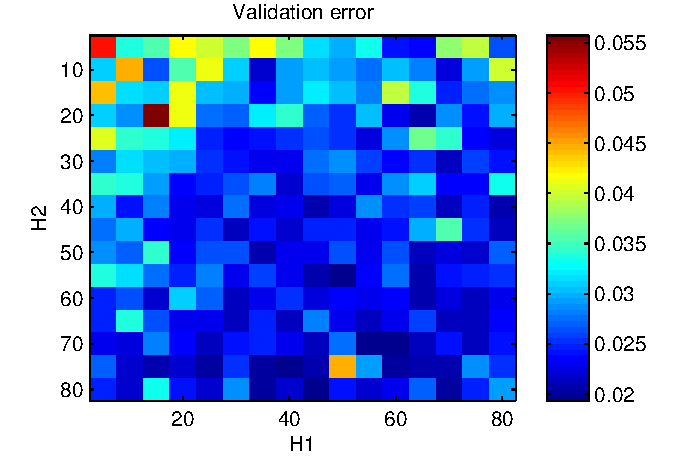
\includegraphics[width=0.6\textwidth]{fig.pdf}
  \caption{Error for various values of $H_1$ and $H_2$.}
  \label{fig:example}
\end{figure}


%%%%%%%%%%%%%%%%%%%%%%%%%%%%%%%%%%%%%%%%%%%%%%%%%%%%%%%%%%%%%%%%%%%%%%%%%
\bibliography{paper} %%%%%%%%%%%%%%%%%%%%%%%%%%%%%%%%%%%%%%%%%%%%%%%%%%%%

\end{document}
